\documentclass{beamer}
\usepackage{beamerthemesplit}
\usepackage{tikz}
\usepackage{ocgx2}
\usepackage{amsmath,amsthm,amssymb,amscd, graphicx,bbm,xcolor}
\usepackage{array}
\usepackage{etoolbox}
\usepackage{mathtools}
\usepackage{subfig}
\usepackage{multirow}
\DeclareMathOperator{\AUC}{AUC}
\DeclareMathOperator{\V}{Var}
\DeclareMathOperator{\cov}{Cov}
\DeclareMathOperator{\corr}{Corr}
\DeclareMathOperator{\sd}{sd}
\DeclareMathOperator*{\argmax}{arg\,max}
\DeclareMathOperator*{\argmin}{arg\,min}
\DeclareMathOperator*{\diag}{diag}
\DeclareMathOperator*{\logit}{logit}
\newcommand{\E}{E}
\renewcommand{\P}{P}
\newcommand{\cind}{\perp \!\!\! \perp}
\newcommand{\X}[1][]{X_{0#1}}
\newcommand{\Y}[1][]{X_{1#1}}
\newcommand{\W}[1][]{W_{#1}}
\newcommand{\w}[1][]{w_{#1}}
\newcommand{\z}[1][]{w_{#1}}
\newcommand{\D}[1][]{D_{#1}}
\renewcommand{\t}[1]{{#1}^T}
\renewcommand{\star}[1]{{#1}^\ast}
\newcommand{\infl}[1][]{\psi_{#1}}
\newcommand{\F}{F}
\newcommand{\G}{G}
% \newcommand{\D}{D}
\newcommand{\m}{m}
\newcommand{\n}{n}
\newcommand{\N}{m+n}
% \newcommand{\risk}{\rho}
\newcommand{\risk}[1][]{\rho_{#1}}
\newcommand{\auc}{\theta}
% \newcommand{\betastar}{\beta_0}
\newcommand{\aucdiff}{\Delta\text{AUC}}
\newcommand{\aucdiffhat}{\hat{\Delta\text{AUC}}}
\newcommand{\kernel}[2]{\{#1 < #2\}}
% \newtheorem{theorem}{Theorem}
\newtheorem{proposition}[theorem]{Proposition}
% \newtheorem{lemma}[theorem]{Lemma}
% \newtheorem{corollary}[theorem]{Corollary}

\setbeamertemplate{navigation symbols}{}
\newcommand{\PreserveBackslash}[1]{\let\temp=\\#1\let\\=\temp}
\newcolumntype{C}[1]{>{\PreserveBackslash\centering}p{#1}}
\graphicspath{{../manuscript/figs/}{../../1/ms/}}
% \graphicspath{{./figs/}}
\makeatletter
\def\input@path{{../manuscript/}}
% \graphicspath{{../../1/ms/}{../../1/ms/figs}}
% \graphicspath{{./figs/}}
\makeatother
\usetikzlibrary{calc}
\mathtoolsset{showonlyrefs=true}
\newtoggle{speaktoggle}
\togglefalse{speaktoggle}
\newcommand{\speak}[1]{
  \iftoggle{speaktoggle}{
    {\tiny{\textcolor{red}{speak: #1}}\normalsize}
  }
  {}
}
% \makeatletter
% \def\input@path{{../manuscript/}}
% % or: \def\input@path{{/path/to/folder/}{/path/to/other/folder/}}
% \makeatother\setbeamertemplate{footline}[frame number]

\title{Nonparametric Estimation of the AUC of an Index with Estimated Parameters}
\author{}
\date{}

\AtBeginSection[] 
{
  \begin{frame}<beamer>
    \frametitle{Outline} 
    \tableofcontents[currentsection]  
  \end{frame}
}

\begin{document}



\begin{frame}
  \titlepage
\end{frame}






\section{Background/Motivation}
\begin{frame}
  \begin{itemize}

  \item medical professionals want to use biomarkers to classify
patients. Combine several characteristics. Usually linear combination
(``index'').

\item e.g., Framingham risk score for 10-year risk of cardiovascular disease, using as covariates  age, sex, LDL cholesterol, HDL cholesterol, blood pressure, diabetes, and smoking. \speak{sand
  ATP III models for 10-year risk of cardiovascular outcomes, Gail model for 5-year risk of
  breast cancer framingham heart score to ((check the purpose in demler)), which
includes smoker status, systolic bp etc.}
  \item Used for policy, insurance etc. \speak{take on a life of their own.  }
\end{itemize}
\end{frame}

% \begin{frame}

%   \begin{itemize}
%   \end{itemize}
% \end{frame}

\begin{frame}

  \begin{itemize}
  \item A good biomarker discriminates well between cases and controls:
    $$P(\beta^T \X < \beta^T \Y),$$
    $\X$ and $\Y$ being independent control and case observations  

  \item Always looking for new indexes. Compare indexes using the difference of AUCs. Typically nested: comparing a known index with another containing an additional covariate.
    $$P(\gamma^T (\X,\X') < \gamma^T (\Y,\Y')) - P(\beta^T \X < \beta^T \Y)$$
\end{itemize}
\end{frame}

\begin{frame}
  Procedure:
  \begin{enumerate}
\item Fit risk models to get coefficients, e.g., $P(\D=1 | \W)=\t\beta \W,P(\D=1 | \W,\W')=\t\gamma (\W,\W')$, to get coefficients $\hat\beta,\hat\gamma$.
\item Then compare observed AUCs
\begin{align}
(\m\n)^{-1} \sum_{i,j}\{\hat\gamma^T (\X,\X')_i < \hat\gamma^T (\Y,\Y')_j\} \\- (\m\n)^{-1}\sum_{i,j}(\hat\beta^T \X[i] < \hat\beta^T \Y[j]\}
\end{align}
\end{enumerate}
Formal test is given in Delong '88.
% \speak{maybe give citations here. what is the relationship between the coef significance and significance of delong test?}
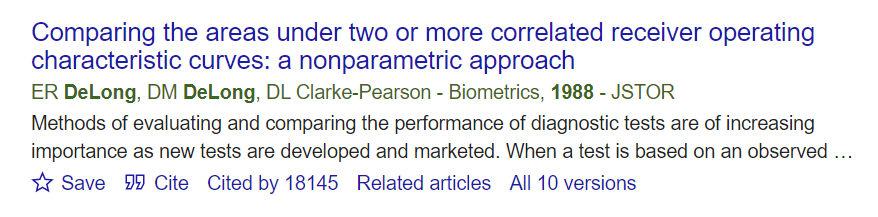
\includegraphics[width=\textwidth]{delong.png}
\end{frame}

\section{Problem}
\begin{frame}

  In the 2000s medical professionals noticed significantly different
  coefficient vectors don't lead to significantly nonzero $\aucdiff$
\begin{footnotesize}
  \begin{itemize}
\item Meigs JB et al. Genotype score in addition to common risk factors for
prediction of type II diabetes. New England Journal of Medicine. 2008; 359(21):2208–2219.

\item Wang TJ et al. Multiple biomarkers for the prediction of
first major cardiovascular events and death. The New England Journal of Medicine. 2006;
355(25):2631–2639.

\item Kattan MW. Judging new markers by their ability to improve predective accuracy. Journal of the
National Cancer Institute. 2003;

\item Cook NR. Statistical evaluation of prognostic versus diagnostic models: Beyond the ROC curve.
Clinical Chemistry. 2008;

\item Hlatky MA et al. Criteria for evaluation of novel markers of cardiovascular risk: A
scientific statement from the american heart association. Circulation. 2009

% \item Cook NR. Use and misuse of the receiver operating characteristics curve in risk prediction.
% Circulation. 2007
\end{itemize}
\end{footnotesize}
Leading some to question the difference in AUC as a useful criterion
\begin{footnotesize}
  \begin{itemize}
\item Tzoulaki I, Liberopoulos G, Ioannisis JPA. Assessment off claims of improved prediction beyond
the Framnigham risk score. JAMA. 2009
\end{itemize}
\end{footnotesize}
\end{frame}

\begin{frame}
By the early 2010s the issue comes to the attenton of biostatisticians 

\vspace{.1in}
% quotes from seshan. ''the baffling observation that use of the
% AUC test to compare nested binary regression models is invalid''
% ``The performance of the AUC test has perplexed other investigators''
\begin{columns}
  \begin{column}{.5\textwidth}
\begin{itemize}
\item Demler, Pencina, D'agonstino 2012: Simulation suggests nested null comparison leads to a degenerate U-stat, non-normal limiting distribution. Not contemplated by Delong's test.
\end{itemize}
\end{column}
\begin{column}{.5\textwidth}
  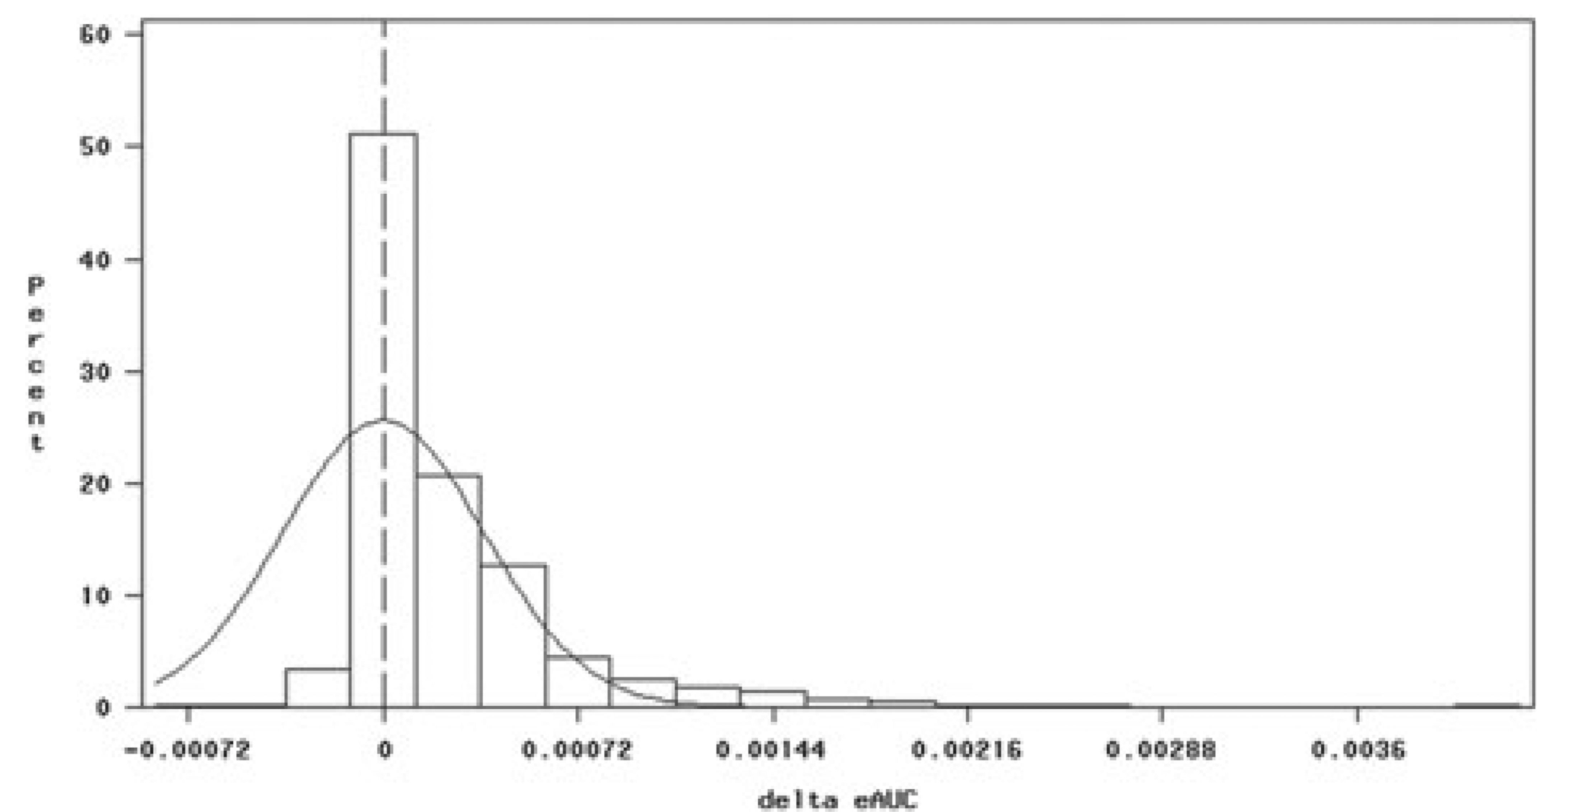
\includegraphics[width=\textwidth]{histogram}
\end{column}
\end{columns}

\begin{itemize}
  \item Seshan, G\"onen, Begg 2013: principal issue is that the observations aren't IID due to the estimated coefficients, violation of the Delong test assumptions
  \end{itemize}
\end{frame}

\begin{frame}
  \begin{itemize}

\item Demler, Pencina, Cook, D'agonstino 2017: theoretical arguments
  that the principal issue is degeneracy of the U-statistic
  
\end{itemize}
\vspace{.2in}
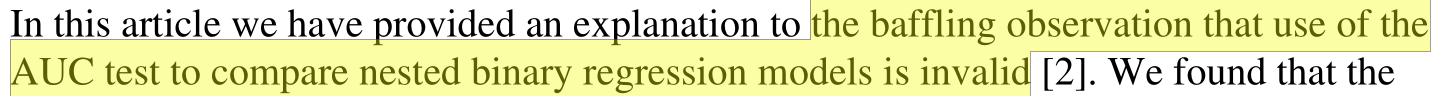
\includegraphics[width=\textwidth]{seshan1}
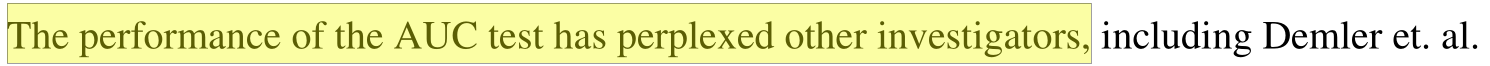
\includegraphics[width=\textwidth]{seshan2}

\end{frame}

\begin{frame}
  Some solutions appear
\begin{itemize}
\item Demler 2011: With gaussian covariates and coeffiicents estimated by LDA or logistic regression, the null of $\aucdiff=0$ is the same as testing for equal Mahalonobis distances, can use an F-test

\item Pepe 2013: the null $\aucdiff=0$ is the same as the risk functions being equal $P(\D=1\mid \W,\W')=P(\D=1\mid \W)$

\item Heller 2017: obtain asymptotic distributions in case coefficient estimation procedure is MRC
\end{itemize}
However,
\begin{itemize}
\item Lee 2021: ``To date, it is remarked that
the asymptotic null distribution of the test statistic computed via the most commonly used MLE of binary
regression parameters is still considered as mathematically intractable in general. At least, Monte Carlo methods
are deemed to be infeasible or otherwise impractical . . .''
\end{itemize}
\end{frame}

\section{Proposed solution for the alternative}

\begin{frame}
  \begin{itemize}
    \item Focus first on the alternative first $\aucdiff\neq 0$: mainly for developing CIs for $\aucdiff$, rather than testing $H_0:\aucdiff=0$


\item Not much advantage gained from the full/reduced relationship
  between the two indexes. Just get an linearization representation for an index
AUC with estimated coeficient, then take difference.
\end{itemize}
\end{frame}

\begin{frame}
  \begin{itemize}
\item strategy in establishing asymptotic normality of U-statistics is to find an asymptotically
equivalent IID representation.

\item In the context of U-statistics usually known
as the hoeffding decomposition. dates to 1940s/50s

% \item ((vander vaart image of hoeffding decomp of mann-whitney))
\end{itemize}
\vspace{.1in}
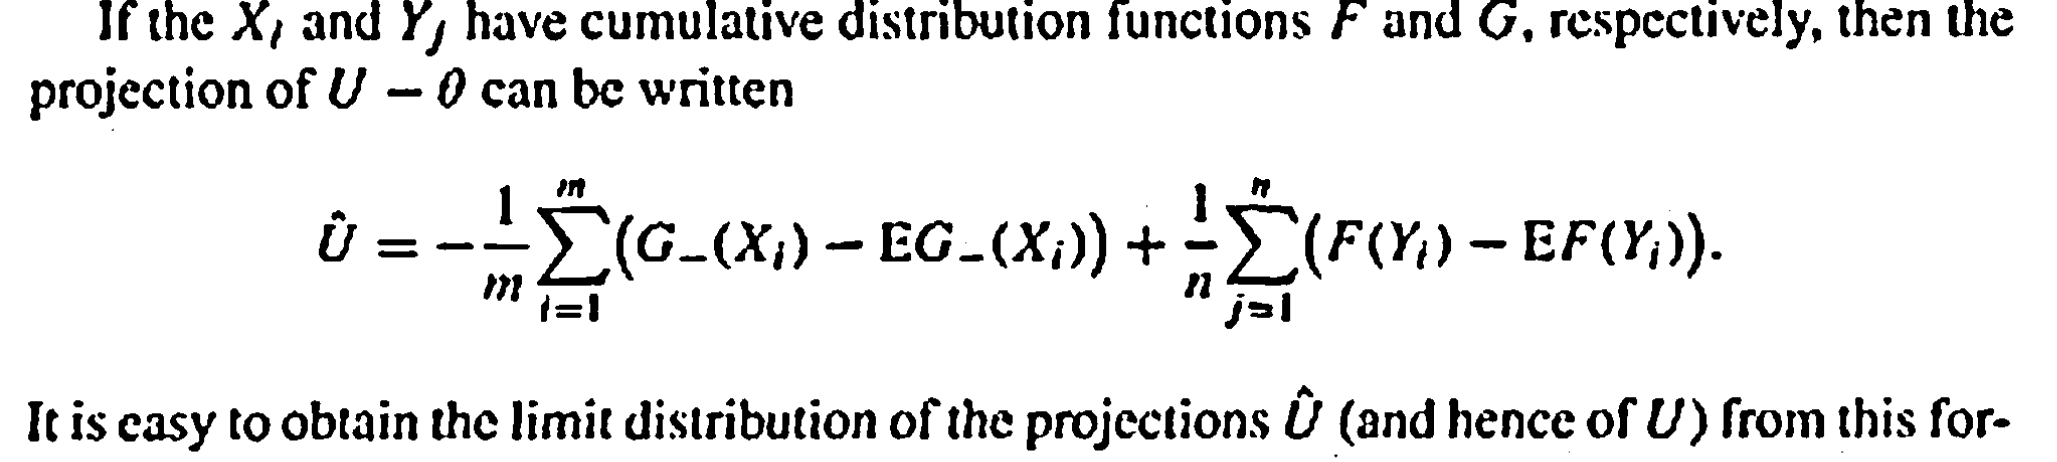
\includegraphics[width=\textwidth]{vdvaart}
\end{frame}

\begin{frame}
 Delong '88: substitute empirical CDFs

  
  \speak{, though not described this
straightforwardly. but important to know that
it's doing the same thing: take a mean, plug in estimators, plug ins
just need to be consistent. will need this: estimating derivative of
estimated function is slow.((then why cant subsitute betahat into hoeffding decomp? that would be an asy estimator of $\theta(\hat F,\hat G,\beta) - \theta(F,G\beta)$.}
\end{frame}


\begin{frame}
Two sources of approximation. IID representation consists of the classical delong rep and an adjustment.

\begin{align}
  &\auc(\hat\F,\hat\G,\hat\beta) - \auc(\F,\G,\star\beta)\\
  &=\auc(\F+\delta\F,\G+\delta\G,\star\beta+\delta\beta) - \auc(\F,\G,\star\beta+\delta\beta) \\
    &+ \auc(\F,\G,\star\beta+\delta\beta)-\auc(\F,\G,\star\beta)
\end{align}
Where \begin{align}
  \auc(F,G,\beta) &= \int\kernel{\t\beta x}{\t\beta y}dF(x)dG(y).
\end{align}
and $\delta\F=\hat\F-\F,$ etc.
\end{frame}

\begin{frame}
\begin{proposition} Given a sample
  $(\W[1],\D[1]),\ldots,(\W[\N],\D[\N])$, and estimator
  $\hat\beta$ based on the sample.
  Assumptions:
  \begin{enumerate}
  \item available influence function for
    $\hat\beta$
  \item $P(\D=0) \in (0,1)$
  \item $\hat\beta\to\star\beta$
  \item   $\auc(\F,\G,\cdot)$ is differentiable at $\star\beta$
  \end{enumerate}
  Assertion:
  $(\N)^{-1/2}(\auc(\hat\F,\hat\G,\hat\beta)-\auc(\F,\G,\star\beta))$
  is asymptotically normal with mean zero, variance can be estimated using the linearization%  with mean zero and variance given by the
  % variance of a term in . This variance may be consistently
  % estimated as $\sqrt{\N}$ times the sample variance of the terms in
  % \eqref{method:iid representation}.
\end{proposition}
% ((add adjustment term somewhere, like the hajek term above??))
% ((mention somewhere derivative needs to be estimated nonparametrically))
In practice, requires non-parametric estimation of a gradient
\end{frame}


\begin{frame}
  \speak{looking for applications of the proposition}
Example: Linear discriminant analysis, but misspecified in that the classes may have different variances
\begin{gather}
  \begin{aligned}
    \W | \D=d \sim N_p(\mu_d,\Sigma_d), d=0,1\\
    \P(\D=1)=1-P(\D=0)=\pi_1
  \end{aligned}
\end{gather}
\end{frame}

\begin{frame}
  A sub-model
  \begin{align}
    % \Sigma_0 = \diag(\epsilon\cdot\mathbbm{
    \Sigma_0=\begin{pmatrix}
      \ddots & & & &\\
      & \epsilon & & & &\\
      & & \ddots & & &\\
      & &  & 2-\epsilon& &\\
      & &  & & \ddots&
    \end{pmatrix},
    \Sigma_1=I,
    \beta=\sqrt{2/p}\mathbbm{1}
  \end{align}
The adjustment term is
  \begin{align}
    |\Sigma_{\pi}^{-1/2}\frac{\partial}{\partial\beta}\auc(\F,\G,\beta)|
    &= \left|\frac{(\pi_1-\pi_0)(1-\epsilon)}{4\sqrt{p\pi\text{e}}}
      \begin{pmatrix}
        \vdots\\
        \pm( 1+(\epsilon-1)\pi_0)^{-1/2}\\
        \vdots        
      \end{pmatrix}\right|
  \end{align}
  which $\to\infty$ as $\pi_0\to 1$ and  $\epsilon\to 0$ simultaneously
\end{frame}

\begin{frame}
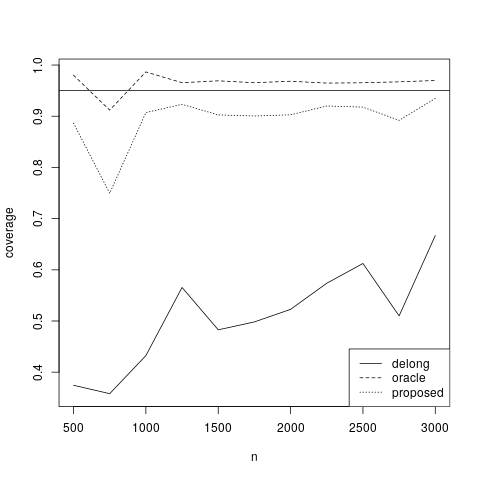
\includegraphics[scale=.5]{../sim/lda/sim}
\end{frame}


\begin{frame}
logit-normal data, well-specified LDA: Delong estimator OK (i.e., no adjustment needed)
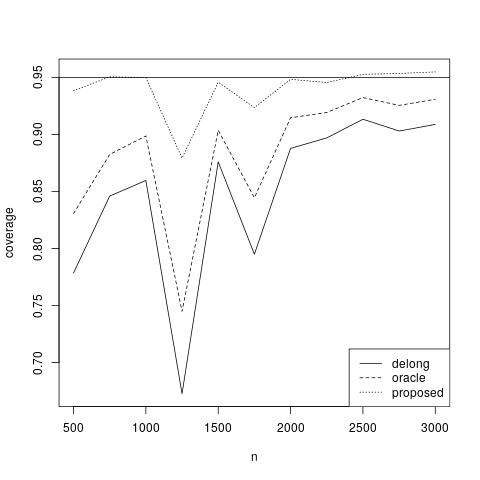
\includegraphics[scale=.45]{../sim/lda/sim_logit}
\end{frame}

\begin{frame}
Why was it so hard to find useful applications of the proposed estimator?
  \begin{columns}
    \begin{column}{.7\textwidth}
\begin{enumerate}
\item the adjustment term is a taylor expansion, the derivative of the AUC at the true coefficient values
%((reproduce adjustment))

\item given covariates $\W$, the ROC curve of the likelihood ratio $w\mapsto f_{\W\mid\D=1}(w)/f_{\W\mid\D=0}(w)$, is at every point maximal \speak{no other ROC curve based on $\W$ exceeds it}

\item the AUC of the likelihood ratio is a stationary point

\item the AUC is invariant to increasing transformations of the data
\end{enumerate}


    \end{column}
    \begin{column}{.3\textwidth}
      % \begin{tikzpicture}
      %   \node[shape=circle,draw=black,font=\tiny] (A) at (0,0) {$NM$};
      %   \node[shape=circle,draw=black,font=\tiny] (Y) at (2,0) {$performance$};
      %   \node[shape=circle,draw=black,font=\tiny] (L) at (1,2) {$talent, etc.$};
      %   \node at (2,1.2) {90\% ?};

      %   \draw [-latex] (A) to [bend left=0] (Y);
      %   \draw [-latex] (L) to [bend left=0] (Y);
      %   \draw [-latex] (L) to [bend left=0] (A);
      % \end{tikzpicture}
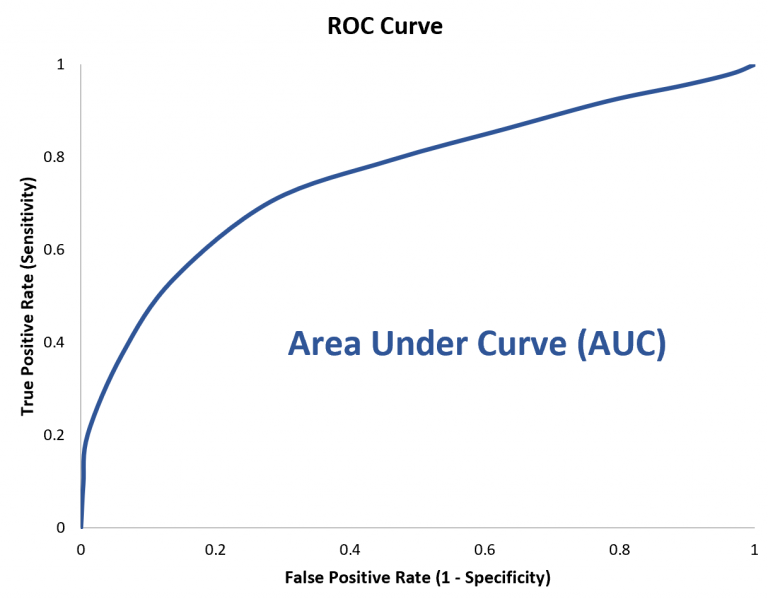
\includegraphics[width=\textwidth]{roc.png}
      
    \end{column}
  \end{columns}
  % \medskip
  % Blazer's edge analyst:  ``No satisfactory conclusions can be found in the realm of `what if'''


\end{frame}


% \begin{frame}
% Why was it so hard to find useful applications of the proposed estimator?

% \begin{enumerate}
% \item the adjustment term is a taylor expansion, the derivative of the AUC at the true coefficient values
% %((reproduce adjustment))

% \item given covariates $\W$, the ROC curve of the likelihood ratio $P(\D=1\mid \W=\w)/P(\D=0\mid \W=\w)$ is at every point maximal; no other ROC curve based on $\W$ exceeds it

% \item the AUC of the likelihood ratio is a stationary point

% \item the AUC is invariant to increasing transformations of the data
% \end{enumerate}

% \end{frame}

\begin{frame}
Binary index model example 
$$ P(\D=1\mid \W) = h(\t\beta \W), \text{$h$ increasing} $$
$$ P(\D=1\mid \W) = \text{expit}\log(P(\D=1\mid \W=\w)/P(\D=0\mid \W=\w)) $$

 so index AUC needs no adjustment
\end{frame}

\begin{frame}
  \begin{itemize}
\item But, there are two AUCs involved in $\aucdiff$% . Even if $...$, the reduced model wouldn't usually be well-specified

\item In many cases correctness of the full
model,
\begin{align}
    \P(\D=1\mid(\W,\W')=(\w,\w')) = h(\t\beta (\w,\w'))\\ \text{ for some }\beta\in\mathbb{R}^{p+q}
\end{align}
implies the reduced model cannot be correct
\begin{align}
  \P(\D=1\mid \W=\w)=\E(h(\t\beta (\w,\w'))\mid \w)\neq h(\t\beta \w)\\ \text{ for any }\beta\in\mathbb{R}^p.
\end{align}
\end{itemize}
\end{frame}

\begin{frame}
  \begin{itemize}
  \item Probit model with gaussian covariates:
    \begin{align}
      \P(\D=1\mid(\W,\W')=(\w,\w')) = \Phi(\t\beta (\w,\w'))\\ \text{ for some }\beta\in\mathbb{R}^{p+q}
    \end{align}
    implies
    \begin{align}
      \P(\D=1\mid \W=\w) = \Phi(\t{\beta'} \w)
    \end{align}
  \item So the adjustment term vanishes
  \item Assertion: For any link, if the covariates are gaussian, the adjustment term vanishes iff the reduced model coefficients are the probit coefficients ($\beta'$ above)
  \item For coefficients obtained under other models, the magnitude of the (nonzero) adjustment term can be controlled by the difference of the coefficients from coefficients obtained under a probit model
  \end{itemize}
  % would for a model such as the probit with gaussian data. then the
  % logistic model is similar, thre is an adjustment but boils down to
  % difference between expit and normal CDF. ((maybe give plot. asy
  % behavior quite different. result: for any link, if the data is
  % gaussian, then the adjustment term only vanishes for the probit
  % coefficients.))

\end{frame}

\section{Remarks on testing the null}

\begin{frame}
  \begin{itemize}
\item nonnormal limit but in some ways null case is simpler. no need for
functional derivative, const terms cancel. can pretransform data with many coef estimation
procedures.

\item nonparametric estimation of a hessian
\end{itemize}
\end{frame}

\begin{frame}

  \begin{itemize}
\item  Difficulty: If the coefficient estimation procedure is
  well-specified, the first-order term in the Taylor expansion
  vanishes, and the limit is non-normal ($1/n$ rate)
\item  If misspecified, the limit is normal ($1/\sqrt{n}$ rate)

\item boundary area
\end{itemize}
\end{frame}


\begin{frame}
  E.g.:
  \begin{itemize}
\item Data follows a logistic model
  $$P(\D=1) = \text{expit}(\beta^T \W)$$
  Two analysts are considering the effect of an additional covariate $\epsilon$ which is in truth just noise
\item One uses logistic regression to fit $\hat\gamma$
  $$\P(\D=1 \mid \W,\epsilon) = \text{expit}(\gamma^T (\W,\epsilon))$$
  The gradient of the AUC at $\star\beta=\star\gamma$ will vanish and the asy distribution will be $O(1/n)$
\item The other uses probit regression: The first-order term will have the form $$(\hat\beta-\hat\gamma)\times (\text{gradient}),$$
  standard asymptotics
\end{itemize}
\end{frame}


\begin{frame}
  Joint work with Alexis Doyle. Nonparametric Estimation of the AUC of an Index with
  Estimated Parameters. Forthcoming. Available at: \texttt{https://haben-michael.github.io/}\\
  \vspace{.7in}
  \centering
  \huge THANK YOU
\end{frame}

\end{document}

- - slide(s) giving list of key papers starting in 2011
should note: non iid observations. degeneracy under the null. show picture.
bootstrap doesnt seem to do well either (maybe a pic of issues). ``perplexing'' etc.




% demler 2011: for lda/logistic regr with normal covariates, testing for improvmenet in discriminaiton is the same as testing for a significants in the coef procedure

% pepe 2013: more generally, can just test if risk functions of the two models are different. null of no diff of risks is the same as null of no diff of aucs.



- proposed solution under alternative



- - write out proposition, along with assumptions.

- - then search for where to apply it




- - collapsibility-type


% monotonic transformatons of likelihood/neyman-pearson. to risk maximized as
% an explanation for why the delong statistic works in many situations.
% auc derivative is maximized when model is well specified,
% for many common models.

% collapsible-type models 

- null situation

